\documentclass[../../main.tex]{subfiles}
\begin{document}
\subsection{Software Architektur Konzept}
Das Konzept der Software Architekur beinhaltet zwei verschiedene Konzepte.
Einerseits gibt es ein Konzept welches mehrere Programme beinhaltet welche über eine Middleware miteinander kommunizieren. \\
Andererseits ein Konzept welches aus verschiedenen Komponenten besteht die über Interfaces miteinander interagieren. \\

\subsubsection{Software Architektur mit verschiedenen Komponenten}
Die Software Architektur besteht aus mehreren Komponenten welche möglichst unabhängig sein sollen und welche mithilfe von Interfaces interagieren.
Es muss sich auf eine Programmiersprache geeinigt werden oder es müssen kleine Wrapper geschrieben werden um beispielsweise
C++ Code von Python Code anzusprechen. Das Testen kann über Unit Tests mit den Interfaces bewerkstelligt werden.
Gemeinsamen Code wird in einer Bibliothek entwickelt.

\begin{figure}[H] %Architektur ohne Middleware
    \centering
    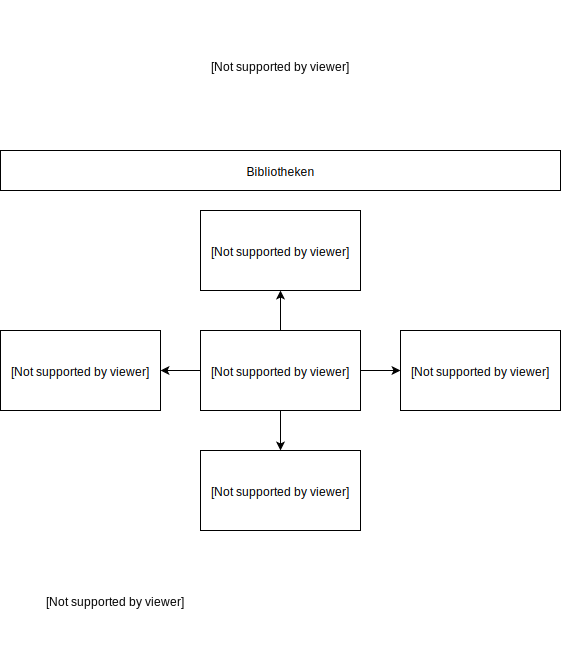
\includegraphics[width=0.6\textwidth]{../../drawings/ArchitekturDiagramm/SW_Architektur.png}
    \caption {Software Architektur Komponenten. Gezeichnet mit https://draw.io}
\end{figure}

\textbf{Legende:}
\begin{itemize}
    \item Die Pfeile visualisieren die Abhängigkeiten innerhalb der Architektur.
    \item Die Abhängigkeit zu den Bibliotheken wurde bewusst weggelassen um das Bild übersichtlich zu halten
\end{itemize}

\subsubsection{Software Architektur mit Middleware}
Die Software Architektur mit Middleware besteht aus mehreren Programmen welche unabhängig gestartet werden.
Sie kommunizieren über eine Middleware miteinander.
Dies ermöglicht den Einsatz von verschiedenen Programmiersprachen und vereinfacht die Implementierung,
da die einzelnen Programme über die Middleware unabhängig getestet werden können.
Um gemeinsamen Code zu teilen wird eine Bibliothek erstellt welche von allen Programmen benutzt werden kann.

\begin{figure}[H] %Architektur ohne Middleware
    \centering
    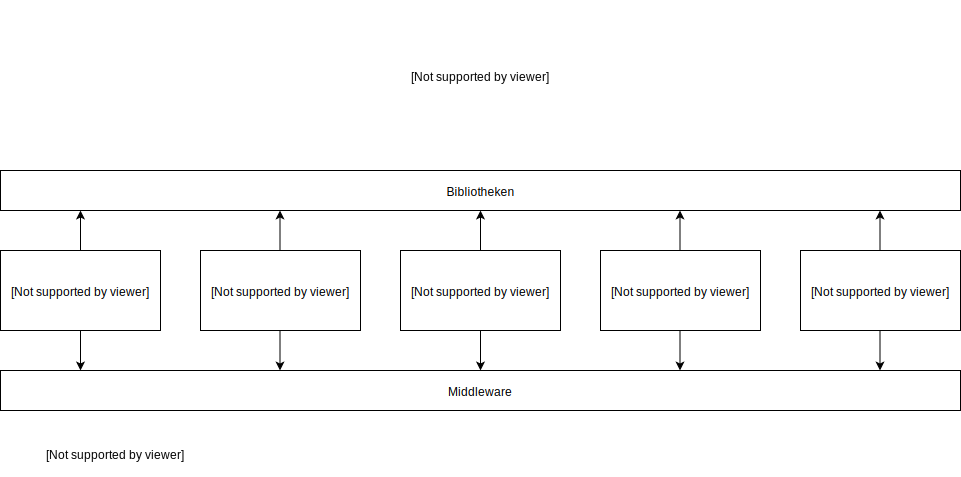
\includegraphics[width=1.0\textwidth]{../../drawings/ArchitekturDiagramm/SW_Architektur_Middleware.png}
    \caption {Software Architektur Middleware. Gezeichnet mit https://draw.io}
\end{figure}

\textbf{Legende:}
\begin{itemize}
    \item Die Pfeile visualisieren die Abhängigkeiten innerhalb der Architektur
\end{itemize}

\subsubsection{Nutzwertanalyse}
\begin{figure}[H]
    \centering
    \includegraphics[width=1.0\textwidth]{../../images/Steuerungssoftware/Nutzwertanalyse_Steuerungssoftware.png}
    \caption {Nutzwertanalyse Steuerungssoftware}
\end{figure}

\subsubsection{Risiken}

\textbf{Risiken Architektur mit Middleware}
    \begin{enumerate}[I]
        \item Schlechte Geschwindigkeit wegen Middleware
        \item Probleme wegen mehrere Prozessen
    \end{enumerate}

    \begin{figure}[H]
        \centering
        \includegraphics[width=0.6\textwidth]{../../images/Steuerungssoftware/Risiko_Steuerungssoftware_Middleware.png}
        \caption {Risikomatrix Steuerungssoftware Middleware}
    \end{figure}

\textbf{Risiken Architektur mit Komponenten}
    \begin{enumerate}[I]
        \item Komplexität weil Monolith
        \item Komplexere Testbarkeit
    \end{enumerate}

    \begin{figure}[H]
        \centering
        \includegraphics[width=0.6\textwidth]{../../images/Steuerungssoftware/Risiko_Steuerungssoftware_Komponenten.png}
        \caption {Risikomatrix Steuerungssoftware Komponenten}
    \end{figure}


%Alte Tabelle vor Nutzwertanalyse
%\subsubsection{Vor- und Nachteile}
%\begin{table}[!h]
%    \begin{tabular}{|l|l|l|ll}
%        \cline{1-3}
%        \textbf{Architektur} & \textbf{Vorteile}                                                                                                        & \textbf{Nachteile}                                                                                             &  &  \\ \cline{1-3}
%        Mit Middleware       & \begin{tabular}[c]{@{}l@{}}-Einfache Testbarkeit\\ -Mehrere Programmiersprachen\\ -Mehrere Prozesse möglich\end{tabular} & \begin{tabular}[c]{@{}l@{}}-Geschwindigkeit\\ -Zusätzliches Know-How \\   für Middleware\end{tabular}          &  &  \\ \cline{1-3}
%        Mit Komponenten      & \begin{tabular}[c]{@{}l@{}}-Geschwindigkeit\\ -Monolith\end{tabular}                                                     & \begin{tabular}[c]{@{}l@{}}-Wrapper benötigt wenn \\   mehrere Programmiersprachen\\ -Testbarkeit\end{tabular} &  &  \\ \cline{1-3}
%    \end{tabular}
%\end{table}

\end{document}